% This is samplepaper.tex, a sample chapter demonstrating the
% LLNCS macro package for Springer Computer Science proceedings;
% Version 2.20 of 2017/10/04
%
\documentclass[runningheads]{llncs}
%
\usepackage{graphicx}
% Used for displaying a sample figure. If possible, figure files should
% be included in EPS format.
%
% If you use the hyperref package, please uncomment the following line
% to display URLs in blue roman font according to Springer's eBook style:
% \renewcommand\UrlFont{\color{blue}\rmfamily}

\usepackage{subfig}
\usepackage{multirow}

\usepackage{hyperref}

\begin{document}
%
% \title{Contribution Title\thanks{Supported by organization x.}}
% \title{Knowledge Discovery - Analysis of players data in FIFA 2019}
\title{OZNAL - Dátová analýza dát hráčov z hry FIFA 19}
%
%\titlerunning{Abbreviated paper title}
% If the paper title is too long for the running head, you can set
% an abbreviated paper title here
%
\author{Timotej Zaťko \and Tomáš Hoffer}
%
\authorrunning{T. Zaťko, T. Hoffer}
% First names are abbreviated in the running head.
% If there are more than two authors, 'et al.' is used.
%
\institute{Fakulta informatiky a informačných technológií STU v Bratislave
Ilkovičova 2, 842 16 Bratislava 4\\
\email{xzatkot1@stuba.sk} \email{xhoffer@stuba.sk}\\
\url{https://www.fiit.stuba.sk/}}
%
\maketitle              % typeset the header of the contribution
%
\begin{abstract}
Táto práca obsahuje analýzu dát hráčov z hry FIFA 19, opis dát a ich charakteristiky. V tejto práci skúmame vzťahy atribútov na predikovaný atribút trhovej ceny hráča a jeho hernú pozíciu na ihrisku.

\keywords{Analýza dát, FIFA 19, Strojové Učenie, Regresia, Klasifikácia}
\end{abstract}

\section{Opis problému a motivácia}

Rozhodli sme sa pre analýzu dát hráčov z hry FIFA 19. V hre sa nachádza veľké množstvo hráčov z rôznych krajín, hrajúcich v rôznych súťažiach. Ich schopnosti v hre by mali odzrkadlovať ich schopnosti z reálneho sveta. Tvorcovia hry sa o to snažia vytvorením herných atribútov, akými sú napríklad rýchlosť šprintu, sila strely, zakončovanie alebo hlavičkovanie ktoré dokázali vyjadriť číselne. V projekte sa budeme snažiť na základe týchto atribútov klasifikovať hráčov do hernej pozície a predikovať ich trhovú hodnotu v hre. Keďže hra hráčom neukazuje vždy trhovú hodnotu hráča, ale len jeho atribúty, náš model môže byť užitočný pri určovaní výšky ponúkanej sumy za prestup hráča pri vyjednávaní v hre. Keďže v reálnom svete schopnosti hráčov (napr. zakončovanie) niesú nijako numericky vyjadrené skúsime využiť to, že v hre vyjadrené sú, na zistenie, ktoré atribúty sú dôležité pre určité herné pozície.

\section{Opis dát s charakteristika dát}
 
% TIMO:
 
% - opis dat
% - najskor high level, pocet atributov, pocer kategorickych, pocet numerickych (pred a po predspracovani)
% - spomenut oblasti atributov - skusit ich zadelit do kategorii
%     - hrac ako clovek - meno, narodnost, vyska, hmotnost, vek
%     - hrac ako futbalista - plat, herne atributy (tych je velmi vela - numericke), Work Rate v utoku/defenzivne, pozicia na ihrisku, body type, medzinarodna reputacia, preferovana noha, sila slabsej nohy
%     - hrac a vztah ku klubu - klub, dlzka kontraktu, typ kontraktu, release claause, joined, jersey number
%     - nerelevantne - photo, face...
    
    
% TIMO:
% sekcia ocistenie dat
% - spomenut predspracovanie - ocistenie dat 
%  - konverzie hodnot - financne hodnoty (tisicky, miliony)
%  - konverzie mier - feet to cm, hmotnost
%  - odstranenie znakov. z numerickycha tributov
%  - konverzia dlzky konktraktu (time)

 
Naša dátová sada obsahuje 18207 záznamov - hráčov, ktorý každý z nich má 87 atribútov. Z toho je 42 numerických a 45 kategorických.
 
\subsection{Očistenie dát} \label{ocistenie_dat}
 
Kvôli analýze bolo treba dátovú sadu, očistiť a urobiť predspracovanie niektorých atribútov. Bolo nutné spraviť nasledovné úpravy -- konverzia a očistenie finančných hodnôt (napr. `\$77.5M`, `\$1K`), konverzia mier (napr. `159lbs`, `5'11`), konverzia časových údajov (napr. `Jan 25, 2019`, `2018`) a rozdelenie niektorých atribútov na viac atribútov - niektoré atribúty obsahovali dva numerické atribúty. Taktiež atribút určujúci pozíciu hráča obsahoval až 38 rôznych herných pozícii, preto sme sa rozhodli tento atribút rozšíriť do ďalších dvoch atribútov v ktorých sme podobné pozície spojili čím vznikli dva atribúty s 13 resp. 4 hodnotami. Po týchto úpravách sa nám počet atribútov zmenil na 129 -- 89 numerických a 40 kategorických atribútov.

Toto veľké množstvo atribútov sme zaradili do nasledovných kategórií, uvádzame k nim aj niektoré atribúty. Atribúty sme rozdelili aj na základe toho či jeho hodnotu musela hra nejakým spôsobom odvodiť z reálneho sveta.

\begin{itemize}
\item \textbf{človek} - meno, národnosť, výška, hmotnosť, vek...
\item \textbf{futbalový hráč (reálny svet)} - názov klubu, číslo dresu, dátum príchodu do klubu, dĺžka kontraktu, plat hráča, hosťovský klub, herná pozícia, preferovaná noha
\item \textbf{futbalový hráč (hra)} - trhová hodnota hráča, triky, pracovitosť v útoku/obrane, vhodnosť na určitú špecifickú pozíciu a potenciálny rast (78 atribútov), medzinárodná reputácia
\item \textbf{futbalové schopnosti hráča určené hrou} (celkovo 34 atribútov) - krátke prihrávky, hlavičkovanie, zakončovanie...
\item \textbf{iné atribúty hry} - logo klubu, vlajka (na základe národnosti), typ postavy (tj. typ herného modelu), typ tváre (tj. kvôli herného modelu)
\end{itemize}

\subsection{Analýza chýbajúcich hodnôt} \label{analyza_chybajucich_hodnot}

% TIMO
% - pozreli sme chybajuce hodnoty a vztahy meczi chybajucimi hodnotami
% - ukazat co sme zistili, dat tam ten insight z deepnotu co je, spomenut dendogram

Ako prvé sme sa pozreli na chýbajúce hodnoty v našej dátovej sade. Početnosti sme vizualizovali stĺpcovým diagramom a vzťahy tepelnou mapou a dendrogramom. Zistili sme, že niektorým hráčom chýbajú hodnoty v atribútoch ako sú klub, plat, dĺžka kontraktu, číslo dresu či výkupná klauzula. Tieto hodnoty chýbajú väčšinou spoločne, o čom sme sa presvedčili v dendrograme a tepelnej mape. Je to aj logické, keďže hráč, ktorý nemá klub nemôže poberať plat alebo mať výkupnú klauzulu v kontrakte. Z našich zistení môžeme konštatovať, že ak hráčovi chýbajú hodnoty v atribúte, väčšinou sa nejedná o chybu v úplnosti dátovej sady.

\subsection{Analýza z pohľadu pozície hráča} \label{analyza_z_pohladu_pozicie}

Analýzu sme ďalej realizovali z pohľadu dvoch atribútov, ktoré sa budeme snažiť predikovať - pozíciu hráča (kategorický atribút) a jeho trhovú hodnotu (numerický atribút). Dátová sada celkovo obsahuje 36 herných pozícií. 

Na základe našich futbalových znalostí sme sa rozhodli zoskupiť podobné pozície do skupín, čím sme znížili počet rôznych hodnôt v atribúte `Position` (Fig. \ref{fig:position_grouping}). Môžeme pozorovať, že triedy nie sú vyvážené.

\begin{figure}%
    \centering
    \subfloat[4 herné pozície(`Position (4)`)]{{ 
        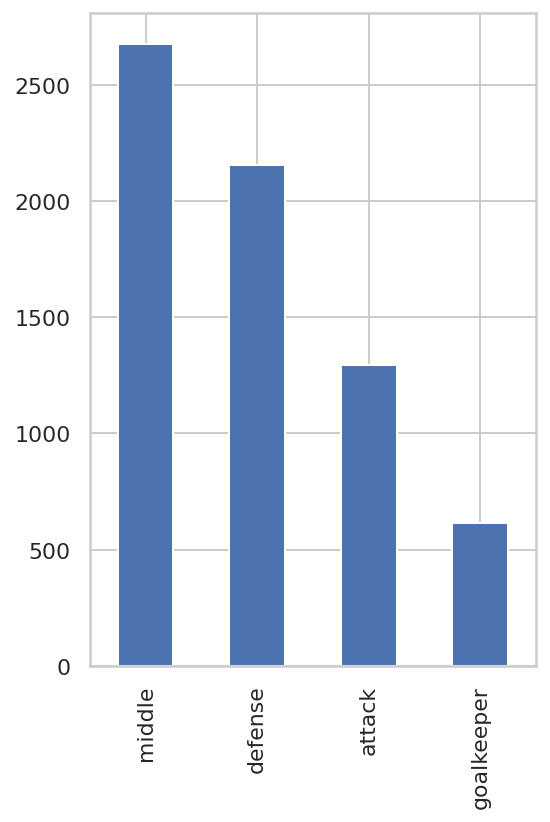
\includegraphics[width=4cm]{images/position_grouping_1}
    }}%
    \qquad
    \subfloat[13 herných pozícií (`Position (13)`)]{{
        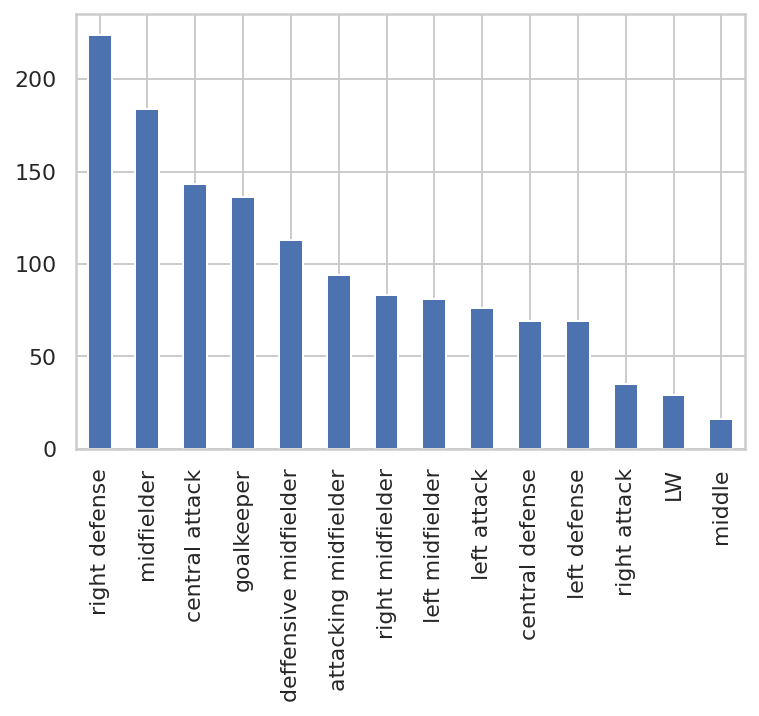
\includegraphics[width=7cm]{images/position_grouping_2}
    }}%
    \caption{Početnosti nových atribútov `Position (4)` a `Position (13)` po zoskupení podobných hodnôt z atribútu `Position`.}%
    \label{fig:position_grouping}%
\end{figure}

Pozíciu sa môžeme pokúsiť predikovať na základe 34 atribútov definujúcich futbalové schopnosti hráča určené hrou. Vizualizovali sme všetky dvojice týchto atribútov a pomocou "scatter plot" -ov  sme hľadali zhluky jednotlivých pozícií. Ako príklad uvádzame vzťah medzi atribútmi `Shot Power` (sila strely) a `Finishing` (zakončovanie), kde môžeme pozorovať jednotlivé zhluky podľa pozície hráča (Fig. \ref{fig:shot_power_finishing_scatter_plot}).

\begin{figure}%
    \centering
    \subfloat[4 herné pozície (`Position (4)`)]{{ 
        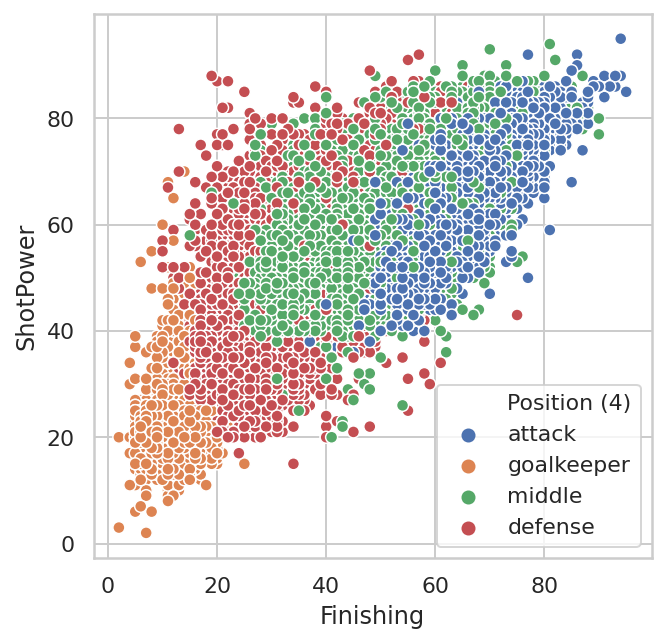
\includegraphics[width=5cm]{images/shot_power_finishing_scatter_plot_position_4}
    }}%
    \qquad
    \subfloat[13 henrých pozícií (`Position (13)`)]{{
        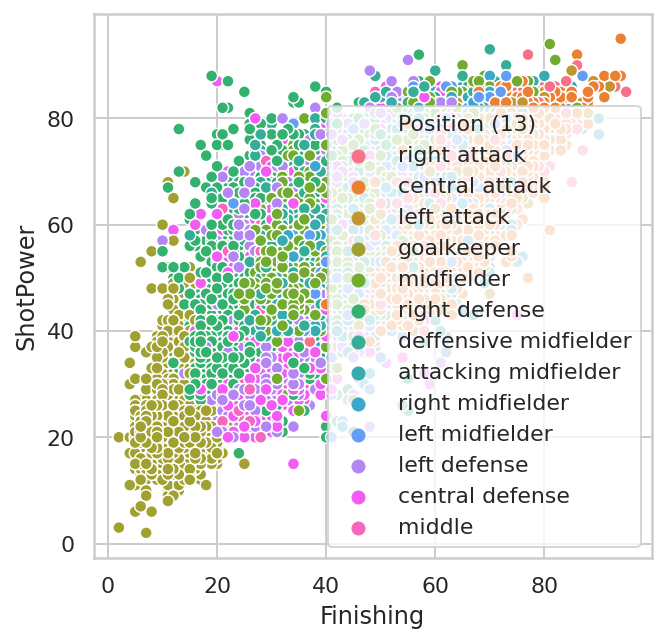
\includegraphics[width=6cm]{images/shot_power_finishing_scatter_plot_position_13}
    }}%
    \caption{Vzťah medzi atribútmi `Shot Power` a `Finishing`. Pre 4 herné pozície sú zhluky zreteľnejšie ako pre 13 herných pozícií.}%
    \label{fig:shot_power_finishing_scatter_plot}%
\end{figure}

Z prieskumnej analýzy tiež vyplýva, že pre konkrétne pozície hráčov sú typické určité čísla dresov. Pre brankárov (angl. goalkeeper) je typickým číslom dresu číslo \textit{1} pričom toto číslo nemá priredený žiaden hráč na inej pozícii. Pre útočníkov (angl. attack) to je \textit{9}, pre obrancov (angl. defense) sú to čísla \textit{2 - 6} a pre stredopoloarov \textit{7}, \textit{8} a \textit{10}. Tento atribút môže byť veľmi dobrý na klasifikáciu pozície hráča, avšak my sa v prvom rade zamieriame na predikciu z herných atribútov. Atribúty, ako napríklad čislo dresu nám môžu úlohu príliš zjednodušiť.

Ďaľšou zaujímavosťou je, že v našej dátovej sade sa nachádzajú prevažne hráči ktorí preferujú pravú nohu, avšak na pozícii ľavého obrancu výrazne prevládajú hráči s preferovanou ľavou nohou. (Fig. \ref{fig:preferred_foot_counts}).

\begin{figure}[htp]
    \centering
    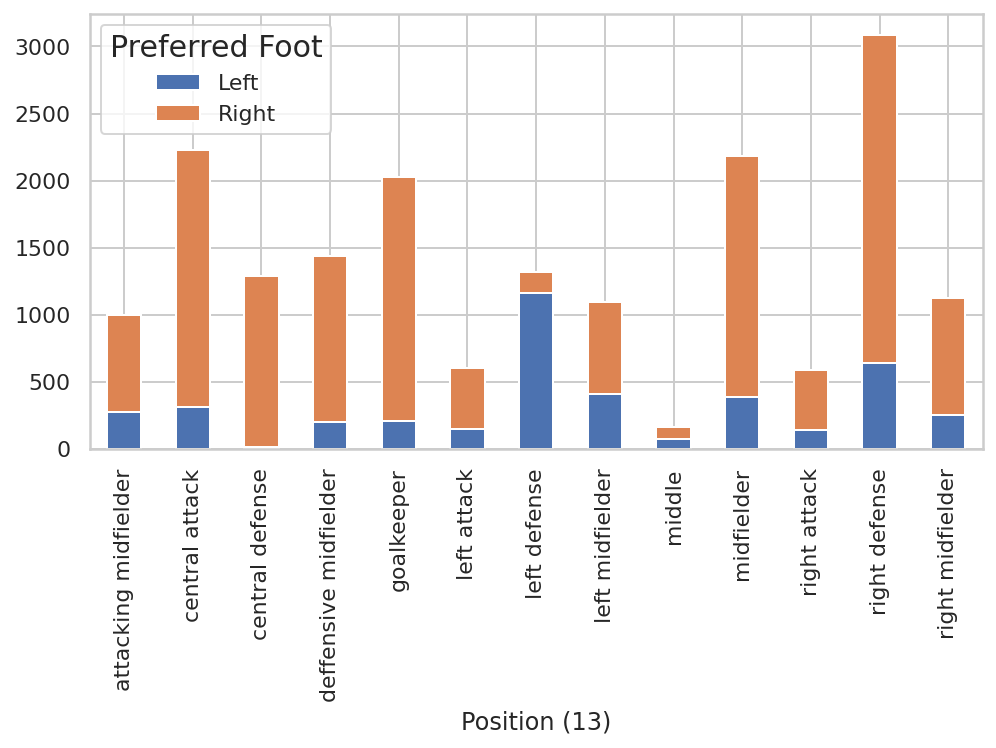
\includegraphics[height=7cm]{images/preferred_foot_counts}
    \caption{Preferovaná noha hráčov podľa hernej pozície.}
    \label{fig:preferred_foot_counts}
\end{figure}

% \begin{figure}[htp]
%     \centering
%     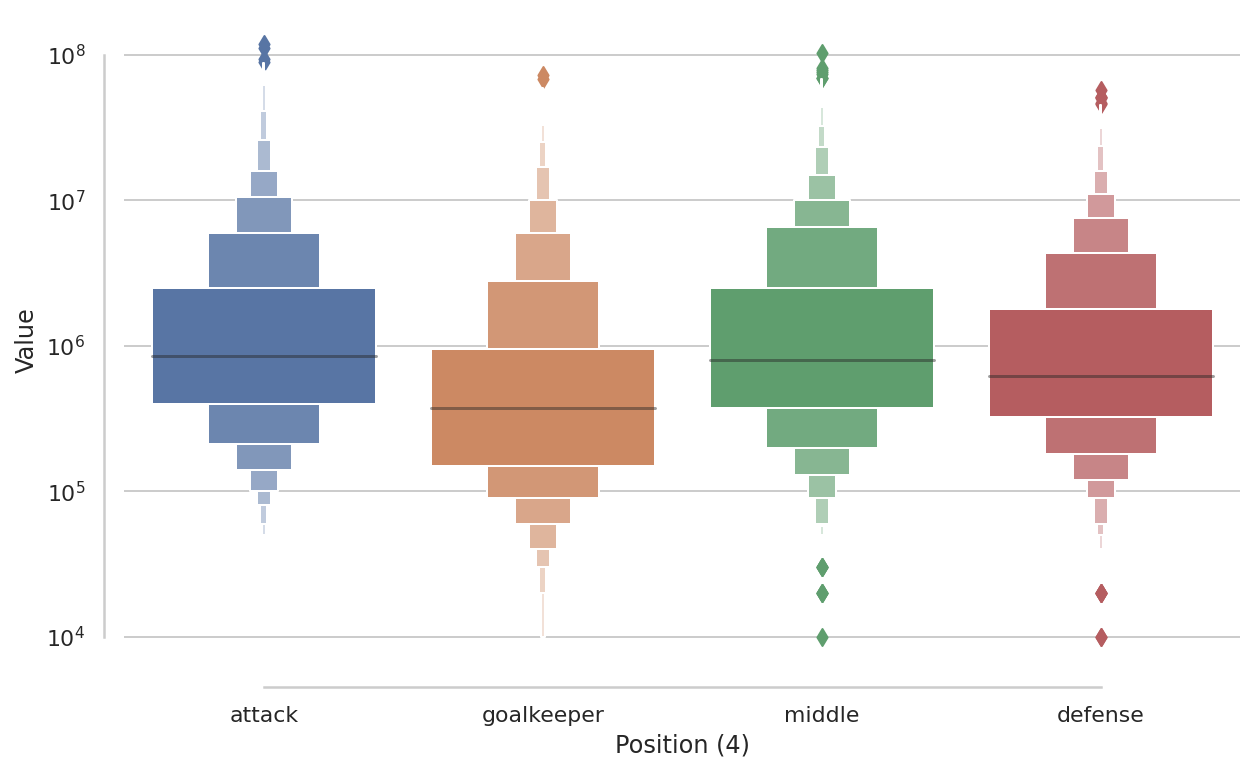
\includegraphics[height=7cm]{images/value_position_boxenplot}
%     \caption{}
%     \label{fig:value_position_boxenplot}
% \end{figure}

\subsection{Analýza z pohľadu trhovej hodnoty hráča} \label{analyza_z_pohladu_trhovej_hodnoty}
Pomocou Pearsonovho korelačného koeficientu sme hľadali korelácie medzi atribútom `Value` a ostatnými numerickými atribútmi. Takmer lineárnu koreláciu (0.99) vykazuje atribút `Release Cause` (Fig. \ref{fig:wage_scatter_plot}). Hráči s vysokou trhovou hodnotou majú v dátovej sade podpísanú zmluvu s vyššou výkupnou klauzulou. Vysokú koreláciu taktiež vykazujú atribúty `Overall` (0.631), `Wage` (0.850) a `International Reputation` (0.656).

\begin{figure}%
    \centering
    \subfloat[Vzťah `Release Cause` voči `Value`.]{{ 
        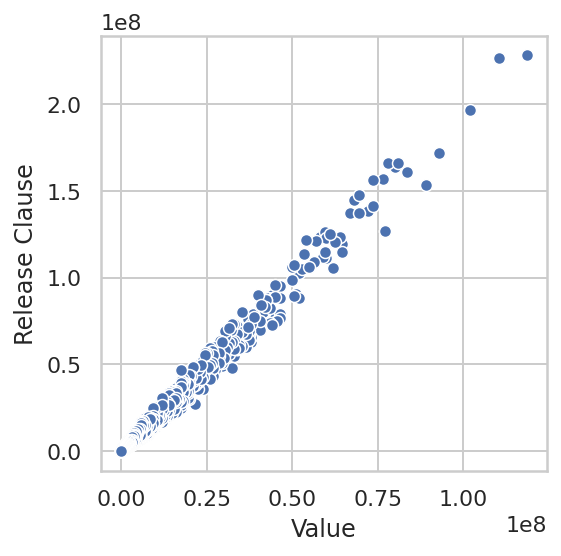
\includegraphics[width=5cm]{images/release_clause_value_scatter_plot}
    }}%
    \qquad
    \subfloat[Vzťah `Wage` voči `Value`.]{{
        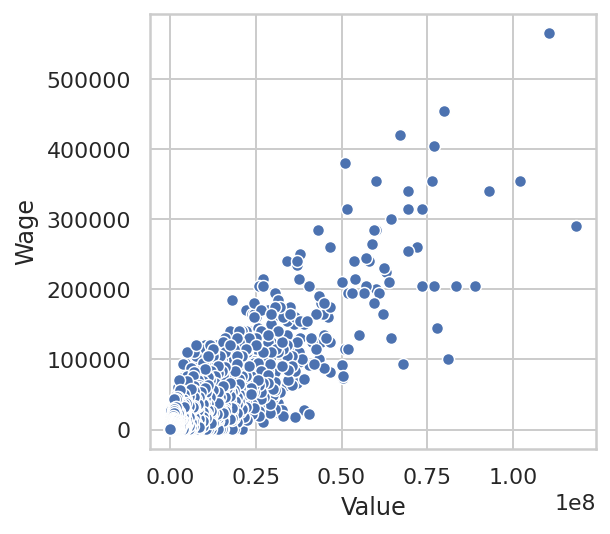
\includegraphics[width=5.5cm]{images/wage_value_scatter_plot}
    }}%
    \caption{Niektoré atribúty vykazujú vysokú mieru korelácie s atribútom `Value`.}%
    \label{fig:wage_scatter_plot}%
\end{figure}


\section{Definovanie úlohy objavovania znalostí \label{task_definition}}

Rozhodli sme sa, že budeme vykonávať nasledujúce úlohy:
\begin{itemize}
    \item predikcia hernej pozície hráča -- všeobecnej (4 triedy), rozšírenej (13 tried) -- \textit{klasifikácia}
    \item predikcia hodnoty hráča (atribút s názvom `Value`) -- \textit{regresia}
\end{itemize}

Obe tieto úlohy budeme realizovať z atribútov určujúcich herné shopnosti hráča a nie zo všetkých atribútov, keďže niektoré atribúty výrazne ovplyvňujú predikovanú premennú a to -- Release Clause - Value; Jersey Number - Position. 

\section{Predpokladaný scenár riešenia (problémy)}

Predpokladáme, že bude potrebné vykonať nasledovné úlohy:
\begin{itemize}
    \item predspracovanie kategorických hodnôt (tj. one-hot encoding)
    \item normalizácia dát
    \item over-sampling
    \item trénovanie modelu
\end{itemize}

Trénovanie modelu zahŕňa výber atribútov (angl. feature selection) a výber a trénovanie modelu. Na úlohu predikcie hodnoty hráča budeme pravdepodobne používať lineárnu regresiu/neurónovú sieť a na určenie hernej pozície hráča rozhodovací strom / náhodný les / SVM / neurónovú sieť.

\section{Predspracovanie dát}

Prvotnému predspracovaniu dát na účely analýzy sme sa venovali v kapitole \ref{ocistenie_dat} kde sme vykonali nasledovné transformácie dát:
\begin{itemize}
    \item Transformácia hodnôt peňažných atribútov (napr. hodnoty `1.2 M`, `200 K` sme transformovali na jednotný numerický tvar)
    \item Dátumové atribúty sme transformovali do jednotného formátu, reprezentovaného UNIX-ovou časovou pečiatkou
    \item Atribúty miery (napr. výška a hmotnosť hráča) sme previedli do rovnakých jednotiek.
    \item Špeciálne pozície hráča boli udávané v tvare reťazca \textit{Value+Grow}. Atribúty špeciálnych pozícií sme rozdelili na dvojice aby nám vznikli numerické atribúty.
    \item Atribút \textit{Work Rate} bol udávaný reťazcom v tvare \textit{Attack/Defense}. Tento atribút sme tiež rozdelili na 2 numerické.
    \item Boolean atribúty udávané reťazcami sme transformovali na numerické 0/1
    \item Vytvorili sme 2 nové atribúty Position(4) a Position(13), ktoré reprezentujú pozíciu hráča po zoskúpení pozícií, opísanom v kapitole \ref{analyza_z_pohladu_pozicie}
    \item Vytvorili sme atribút \textit{Contract length}, ktorý reprezentuje dĺžku aktuálne podpísanej zmluvy hráča 
\end{itemize}

Kategorické atribúty sme transformovali metódou "One-Hot Encoding". Numerické atribúty sa nachádzali v rôznych rozsahoch a jednotkách (napríklad hmotnosť v lb, výška v cm, rôzne schopnosti hráča v rozsahu $<0,100>$). Rozhodli sme sa ich normalizovať do jednoetného intervalu $<0,1>$.

\subsection{Chýbajúce hodnoty}

V kapitole \ref{analyza_chybajucich_hodnot} sme opísali dôvod výskytu chýbajúcich hodnôt. Chýbajúce hodnoty opísané v kapitole \ref{analyza_chybajucich_hodnot} považujeme za opodstatnené a nebudeme ich nahrádzať. Tj. dané hdonoty chýbajú pretože majú chýbať a nie preto, že by boli dáta neúplné.

\subsection{Vychýlené hodnoty}

Rozdelenie číselných hodnôt v dátovej sade sme podrobne analyzovali a vizualizovali. Vychýlené hodnoty sú iba v niektorých atribútoch. 

\subsection{Problém nevyváženosti tried \label{class_imbalance_problem}}

Pri zoskúpení všetkých pozícií do 13 tried sme odhalili nevyváženosť jednotlivých tried (Fig.\ref{fig:position_grouping}), čo by mohlo negatívne ovplyvniť presnosť predikcie. Tento problém sme sa rozhodli riešiť metódou nazývanou \textit{oversampling} a konkrétne algoritmom SMOTE \cite{AlbertoFernandez2018}, ktorý vytvára syntetické inštancie minoritných tried/y pomocou lineárnej kombinácie reálnych inštancií.

\section{Výber atribútov}

Predikciu pri oboch typoch úloh budeme realizovať pomocou 34 atribútov definujúcich futbalové schopnosti hráča určené hrou. Využijeme tiež demografické údaje, napr. výšku, hmotnosť a vek. K tejto základnej množine atribútov sme sa dopracovali na základe doménovej znalosti a rozsiahlej prieskumnej analýzy. V častiach \ref{analyza_z_pohladu_pozicie} a \ref{analyza_z_pohladu_trhovej_hodnoty} sa venujeme výberu týchto atribútov a opisujeme dôvody, prečo sme niektoré atribúty do tejto množiny nezahrnuli.
% -- toto uvidime ci budeme robit, mame uz toho aj tak dost
% V druhej etape riešenia vyskúšame úlohy predikcie realizovať s využitím všetkých atribútov a úspešnosti modelov porovnáme. Očakávame mierny nárast úspešnosti pri použití všetkých atribútov.
Pri riešení klasifikačnej úlohy rozšírime základnú sadu atribútov o atribúty \textit{Preferred Foot}, \textit{Work Rate Attack} a \textit{Work Rate Defense}. Pri regresnej úlohe využijeme dopočítaný atribút \textit{Contract Length} a využijeme tiež medzinárodnú reputáciu hráča (\textit{angl. International reputation}).
Množinu vybraných atribútov sa pravdepodobne ešte pokúsime zredukovať (angl. feature selection). V závislosti od modelu zvolíme konkrétny prístup. Niektoré modely podporujú tzv. \textit{feature importances}. Pri modeloch, ktoré to nepodorujú môžeme použiť rekurzívnu elimináciu atribútov alebo prírodou inšpirované algoritmy, ktoré v tejto oblasti dosahujú veľmi dobré výsledky \cite{zawbaa2018large}.

\section{Príbuzná práca}

V našej doméne (avšak na dátach zo staršej verzie hry) Soto-Valero, C. \cite{RICYDE1165} zisťoval, ktoré atribúty sú dôležité pre jednotlivé herné pozície. Využil PCA na zredukovanie dimenzionality zo všetkých herných atribútov a následne zhlukovaním klasifikoval hráčov do jednotlivých herných pozící. Následne pomocou algoritmu \textit{Gradient tree boosting} ohodnotil dôležitosť jendotlivých atribútov. Na klasifikovanie využil takzvané učenie bez učiteľa, čím sa jeho práca líši od tej našej.

Nazim R. a spol. sa snažia predikovať pozíciu hráča na základe podobných atribútov, avšak využívajú dátovú sadu zo športovej školy  \textit{Bukit Jalil Sports School}. Na klasifikáciu využívajú bayesovské siete, rozhodovacie stromy a algoritmus najbližšieho suseda. Hráči boli klasifikovaní do 10 tried. Vzhľadom na to, že dátova sáda obsahovala len 100 prvkov sa autori rozhodli použiť \textit{"leave-one-out"} validáciu \cite{razali2017}.  

Yaldo L. a Shamir L. sa snažia riešiť problém predikcie týždenného platu futbalového hráča pomocou 8 rôznych algoritmov strojového učenia na podobnej dátovej sade FIFA z roku 2016 \cite{yaldo2017}. Autori na predikciu využili napríklad aditívnu regresiu či rozhodovacie stromy. Platy hráčov sú predikované na základe ich pozície, ale aj atribútov hry, ktoré charakterizujú ich schopnosti.
Zaujímavým zistením je fakt, že platy hráčov nezávisia len od ich schopností a pozície hráča, ale aj celkovej reputácie a jeho popularity. Známy hráč L. Messi by napríklad pri predikcii len na základe jeho schopností nedosiahol ani polovičný plat. Rozhodli sme sa teda medzinárodnú reputáciu hráča zahrnúť medzi črty použité na predikciu.
Autori používajú Piersonov korelačný koeficient (CC) a priemernú absolútnu odchýlku (MAE) na meranie úspešnosti.


\section{Výber metrík pre evaluáciu úspešnosti}

\paragraph{Klasifikácia} -- keďže klasifikujeme do 4 resp. 13 tried, ktoré sú nevyvážené, budeme sledovať metriky \textbf{f1 micro} a \textbf{f1 macro}.
Táto metrika je harmonickým priemerom \textit{precision} a \textit{recall} \cite{opitz2019macro}.
Nás zaujíma predovšetkým varianta \textbf{micro}, keďže máme nevyvážené triedy a chceme aby metrika brala do úvahy početnosti tried (tj. náš model nemusí byť taký dobrý v klasifikácii minoritných tried). Budeme tiež sledovať aj variantu \textbf{macro}, ktorá berie do úvahy všetky triedy rovnako.

\paragraph{Regresia} -- pri regresii budeme sledovať metriku s názvom \textbf{RMSE} (Root Mean Sqaure Error).

\section{Opis použitých algoritmov}

\subsection{Predikcia pozície hráča (klasifikácia)}

\paragraph{Rozhodovací strom} --
klasifikátor založený na stromovej štruktúre. Uzly reprezentujú test vykonaný nad atribútom inštancie a vetvy reprezentujú možné výsledky testu. Rozhodovací strom pri klasifikácii začína v koreni a postupne prechádza cez jednotlivé ulzy až k listu, ktorý reprezentuje výsledok klasifikácie (triedu). 

\subsection{Predikcia trhovej hodnoty hráča (regresia)}

\paragraph{Lineárna regresia} --
algoritmus, ktorý sa pokúša modelovať vzťah medzi dvoma premennými pomocou lineárnej funkcie. Rovnica lineárnej regresie má tvar $Y = kX + q$, kde \textit{Y} a \textit{X} sú závislé premenné, \textit{q} udáva posun a \textit{k} udáva sklon funkcie. Algoritmus je vhodný pri riešení regresných úloh, pri ktorých modelujeme lineárny vzťah medzi premennými. Vzájomnú koreláciu je vždy vhodné vopred overiť pomocou Pearsonovho korelačného koeficientu. 

\subsection{Skupinové učenie (angl. "ensemble learning")}

\paragraph{Náhodný les} --
klasifikátor/regresor, ktorý využíva viacero rozhodovacích stromov, ktoré sú trénované nezávisle a každý pri klasifikácii dostane 1 hlas. Náhodný les následne vyberie triedu s najvyším počtom hlasov. Výhodou algoritmu je tiež zabránenie korelácie medzi jednotlivými rozhodovacími stromami vďaka využitiu "bagging" metódy. Rozhodovacie stromy sú trénované na množinách dát, ktoré vznikajú výberom s nahradzovaním (angl. "selection with replacement"). Vďaka tejto metóde výberu vznikajú rozhodovacie stromy rôznych šírok a hĺbok a práve ich rôznorodosť prispieva k úspešnosti algoritmu náhodného lesa.

\paragraph{Adaboost} --
klasifikátor/regresor založený na lineárnej kombinácii viacerých tzv. slabých klasifikátorov/regresorov, trénovaných na iteratívne modifikovaných dátach ("boosting" iteráciách). Iterácie pozostávajú z aplikácie váh \(w_1, w_2, ... w_N\), pričom N reprezentuje počet prvkov. Počas každej iterácie sú váhy nesprávne klasifikovaných prvkov z predchádzajúcej iterácie zvýšené, resp. znížené pri správnej klasifikácii. Pozorovania, ktoré je náročné správne klasifikovať postupne dostanú vysokú váhu a slabé klasifikátory sa pri ďalšom trénovaní zameriavajú na tieto pozorovania. Predikcie slabých klasifikátorov sú nakoniec kombinované a použité na finálnu predikciu.

\paragraph{Gradient tree boosting} --
klasifikátor/regresor využíva rozhodovacie stromy ako slabé klasifikátory/regresory. Rozhodovacie stromy sú postupne vytvárané a pridávané do množiny použitých slabých klasifikátorov s využitím metódy klesajúceho gradientu (angl. "gradient descent") na minimalizáciu chybovej funkcie. 

\paragraph{Voting classifier/regressor} --
klasifikátor/regresor kombinujúci výsledky viacerých rôznych klasifikátorov/regresorov. Použitie algoritmu je vhodné napríklad v prípade, keď máme viacero úspešných modelov na vyváženie ich slabostí. Metóda "hard voting" priradzuje každému modelu hlas s rovnakou váhou. Metóda "soft voting" umožňuje priradenie váhy hlasom jednotlivých modelov.  

\paragraph{Stacked generalization} --
klasifikátor/regresor kombinujúci výsledky viacerých modelov. Výsledky modelov sú vstupom finálneho modelu, ktorý je trénovaný s využitím krížovej validácie. 


\section{Experimenty}

\subsection{\label{classification} Predikcia pozície hráča (klasifikácia)}

Úlohu sme sa v prvej etape rozhodli riešiť pomocou viacerých jednoduchých modelov. Klasifikácia hráča do 4 pozícií už pri základných nastaveniach modelov vykazovala vysokú úspešnosť \ref{tab:f1_position_4}. Model sa najviac mýlil pri klasifikácii do triedy \textit{middle}. Je to pochopiteľné, keďže stredopoliari sú "medzi" útočníkmi a obrancami \ref{fig:confusion_matrix_position_4}. 

Pri klasifikácii do 13 tried pozície je úspešnosť jednoduchých modelov významne nišia a niektoré triedy jednotlivé modely dokonca vôbec nepredikovali.

% https://tablesgenerator.com/#
\begin{table}[]
    \begin{tabular}{|l|rrrrrr|rr}
    \hline
    \multicolumn{1}{|c|}{\multirow{2}{*}{Model}} & \multicolumn{6}{c|}{Position (4) -- f1 skóre}                               & \multicolumn{2}{l|}{Position (13) -- f1 skóre} \\
    \multicolumn{1}{|c|}{}                       & Attack & Defense & GK         & Middle & Micro & \multicolumn{1}{l|}{Macro} & Micro       & \multicolumn{1}{l|}{Macro}       \\ \hline
    Rozhodovací strom                            & 0.74   & 0.87    & 1          & 0.76   & 0.81  & 0.84                       & 0.55        & \multicolumn{1}{r|}{0.42}        \\
    Logistická regresia                          & 0.82   & 0.94    & 1          & 0.87   & 0.87  & 0.90                       & 0.71        & \multicolumn{1}{r|}{0.53}        \\
    SVM                                          & 0.81   & 0.93    & 1          & 0.84   & 0.88  & 0.89                       & 0.66        & \multicolumn{1}{r|}{0.44}        \\
    Náhodný les                                  & 0.81   & 0.93    & 1          & 0.86   & 0.89  & 0.89                       & 0.68        & \multicolumn{1}{r|}{0.50}        \\ \hline
    \end{tabular}
    \\
    \caption{\label{tab:f1_position_4} Úspešnosti jednoduchých modelov pri predikcii `Position 4` a `Position 13`. Pre predikciu štyroch herných pozícií zobrazujeme aj metriku \textbf{f1} pre jednotlivé pozície. V oboch prípadoch bola najlepšia logistická regresia a náhodný les.}
\end{table}

\begin{figure}%
    \centering
    \subfloat[Matica zmätenia pre model náhodny les.]{{ 
        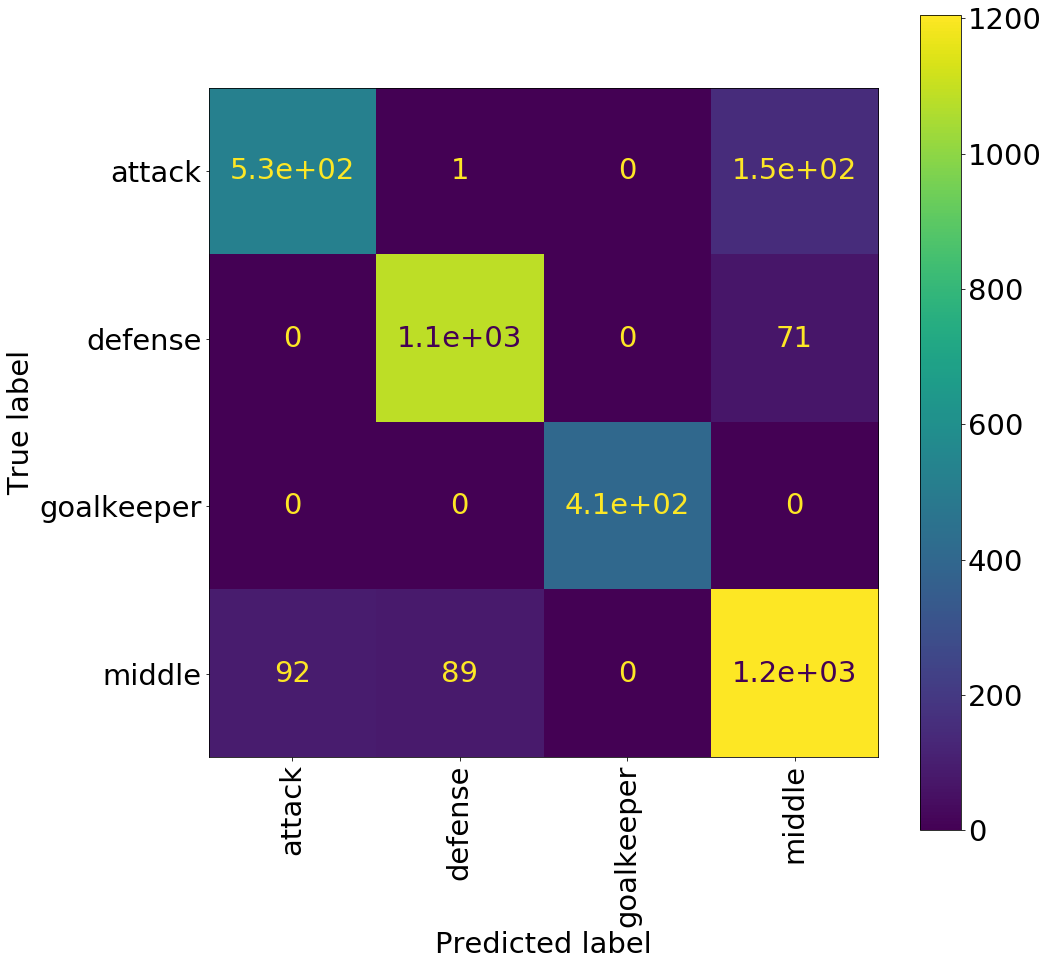
\includegraphics[width=5.5cm]{images/confusion_matrix_position_4_random_forest}
    }}%
    \qquad
    \subfloat[Matica zmätenia pre model logistickej regresie.]{{
        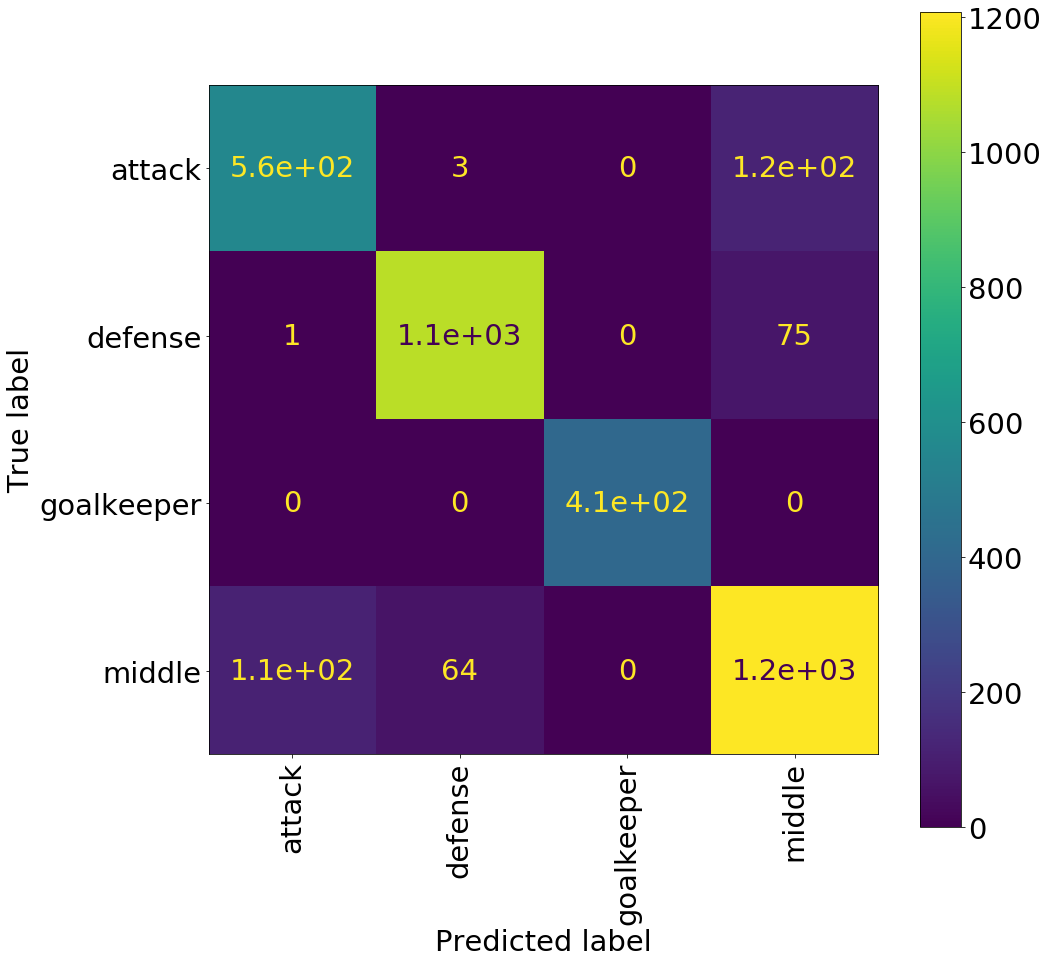
\includegraphics[width=5.5cm]{images/confusion_matrix_position_4_logistic_regression}
    }}%
    \caption{Matice zmätenia pre dva z našich natrénovaných modelov, môžeme si všimnúť že model robí chyby pri klasifikácii do triedy \textit{middle}.}%
    \label{fig:confusion_matrix_position_4}%
\end{figure}

\subsection{\label{regression} Predikcia trhovej hodnoty hráča (regresia)}

Na riešenie tejto úlohy sme využili lineárnu regresiu. V tejto úlohe sa nám zatiaľ nepodarilo dosiahnuť výraznejšie výsledky (Obr. č.\ref{fig:value_pred_true_scatterplot}).

\begin{figure}[htp]
    \centering
    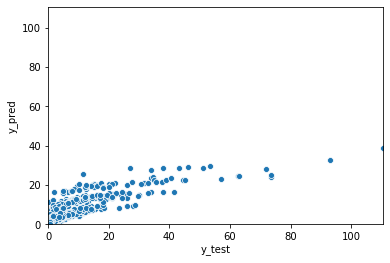
\includegraphics[height=5cm]{images/value_pred_true_scatterplot}
    \caption{Predikované hodnoty hráčov a reálne hodnoty hráčov v miliónoch. Zatiaľ sa nám nepodarilo dosiahnúť lepšie výsledky (\textit{RMSE = 3,560331}).}
    \label{fig:value_pred_true_scatterplot}
\end{figure}

\subsection{Oversampling}

Keďže pri našej klasifikačnej úlohe sú jednotlivé triedy nevyvážené (Sekcia \ref{class_imbalance_problem}) pokúsíli sme sa zvýšiť početnosti minoritných tried. Vyskúšali sme minoritné triedy dovzorkovávať náhodne a zároveň metódou SMOTE a jej variáciami (SVM-SMOTE, BorderlineSMOTE). Tiež sme skúšali rôzne kombinácie hyperparamet-rov týchto metód.
Ako model s pouižili náhodný les, keďže zo všetkých modelov sa trénoval najrýchlejšie a patril medzi najlepšie modely (Tab. \ref{tab:f1_position_4}). Pri klasifikácii do `Position 4` a `Position 13` oversampling modely výrazne nezlepšil.
Pri všetkých modeloch sa zlepšila metrika \textit{f1 macro} a zas shoršila \textit{f1 micro}, tj. model sa zlepšil na klasifikácii minoritných tried na úkor mierneho zhoršenie klasifikácie tých majoritných.
Najlepší model s použitím SMOTE bol lepší o 2 percentuálne body v metrike \textit{f1 macro} a 0.4 percentualného bodu horší v metrike \textit{f1 micro}.
Použitím oversampling-u sme dosiahli iba mierne zlepšenie v klasifiácii.

\subsection{Výber atribútov (angl. feature selection)}

Jednotlivé atribúty sme zatiaľ vyberali iba na základe doménových znalostí a podľa nami definovanej úlohy objavovania znalostí (Sekcia \ref{task_definition}). Keďže je týchto atribútov stále veľa, pokúsili sme sa ich zredukovať aby sme mali jednoduchší a ľahšie interpretovateľný model. Vyskúšali sme niekoľko spôsobov, a to konkrétne: odstránenie atribútov s nízkou varianciou, výber atribútov na základe jednorozmerných štatistických testov (angl. "univariate feature selection"), rekurzívnu elimináciu atribútov, výber na základe ich dôležitosti pre model (angl. "feature importances"). V rámci týchto metód sme skúšali rôzne parametre a výber atribútov sme vykonávali pre klasifikačnú úlohu (klasifikátor - náhodný les) a aj pre regresnú úlohu (lineárna regresia).

Výber atribútov výrazne nezlepšil úspešnosť modelu, ale ani nezhoršil. Použitím polovice zo všetkých atribútov sme dosiahli rovnako dobré výsledky ako keby sme ich použili všetky (Obr. \ref{fig:feature_selection_classification_position}). Pri regresii bol tento trend podobný.

Výberom atribútov sa nám podarilo natrénovať jednoduchšie modely s podobnou úspešnosťou ako bez výberu atribútov.

\begin{figure}%
    \centering
    \subfloat[Úspešnosť pri klasifikácii `Position 4` podľa počtu použitých atribútov]{{ 
        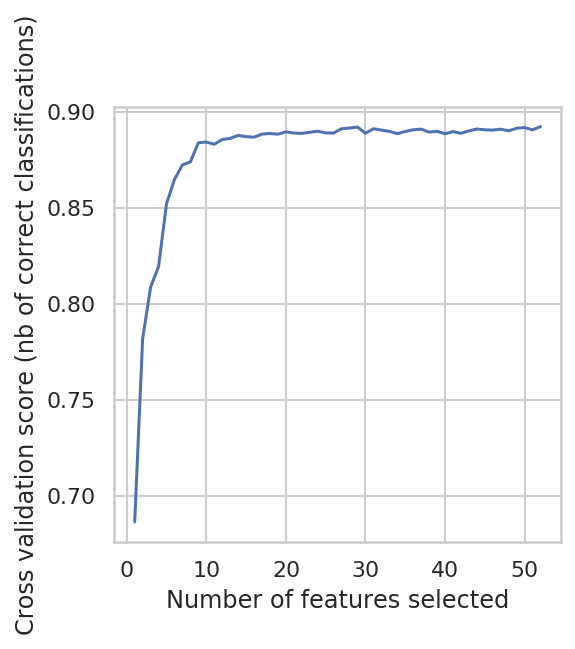
\includegraphics[width=5.5cm]{images/feature_selection_classification_position_4}
    }}%
    \qquad
    \subfloat[Úspešnosť pri klasifikácii `Position 13` podľa počtu použitých atribútov]{{
        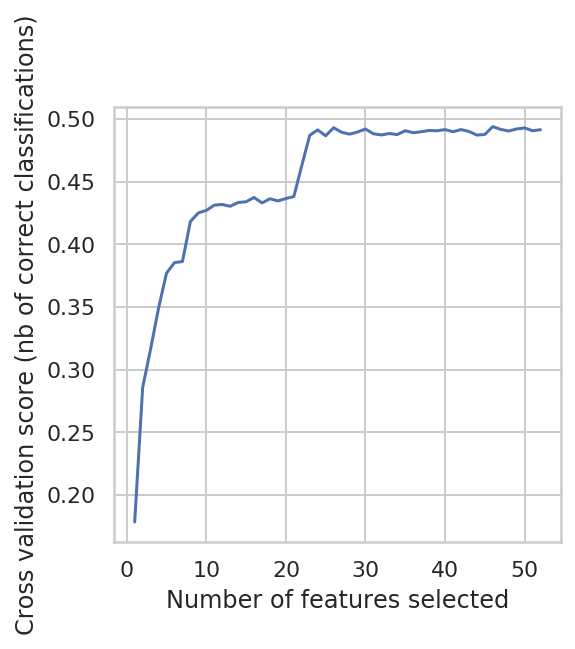
\includegraphics[width=5.5cm]{images/feature_selection_classification_position_13}
    }}%
    \caption{Úspešnosti pri klasifikácii podľa počtu použitých atribútov. Graf vznikol použitím rekurzívnej eliminácie s krížovou validáciou (\textit{k=2}) na klasifikátore náhodný les.}%
    \label{fig:feature_selection_classification_position}%
\end{figure}

\subsection{Ensemble}

Vyskúšali sme niektoré ensemble metódy, pomocou ktorých sa nám podarilo dosiahnuť ešte lepšie výsledky ako sme dosiahli doteraz. Vyskúšali sme AdaBoost, Gradient Tree Boosting (ďalej GDT), Voting (hard a soft) kde sme použili logiskickú regresiu, rozhodovací strom a SVM. Ďalej sme vyskúšali metódu stacked generalization, kde sme použili náhodný les, AdaBoost a GDT. S metódami sme viac do hĺbky neexperimentovali. Pri prvotých experimentoch bol najlepší GDT s tým, že jeho trénovanie trvalo pomerne krátko, čo nám umožnilo použiť ho aj pri hyper-parameter tunningu.

Pri regresnej úlohe spomedzi použitých metód bol výrazne najlepší Gradient Tree Boosting s pomerne krátkym časom trénovania.

\subsection{Hyper-parameter tunning}

Pri oboch úlohách sme realizovali hyper-parameter tunning pomocou algoritmu Grid Search na metóde Gradient Tree Boosting. V oboch prípadoch sme optimalizovali nasledujúce hyper-parametre - \textit{min samples leaf}, \textit{number of estimators}, \textit{max depth}, \textit{min samples split} a \textit{subsample} (tieto parametre sú bližšie vysvetlené \href{https://scikit-learn.org/stable/modules/generated/sklearn.ensemble.GradientBoostingRegressor.html}{tu}). Dosiahnuté výsledky sme vizualizovali pomocou tepelných máp. Keďže je grid search najmenej optimálna metóda hľadania hyper-parametrov, prehľadávali sme pomerne malý priestor parametrov. Taktiež sme sa pokúšali hľadať najoptimálnejšie dvojice parametrov alebo sme optimalizovali iba jeden parameter. Aj preto výsledky nie sú výrazne lepšie.

\begin{figure}[htp]
    \centering
    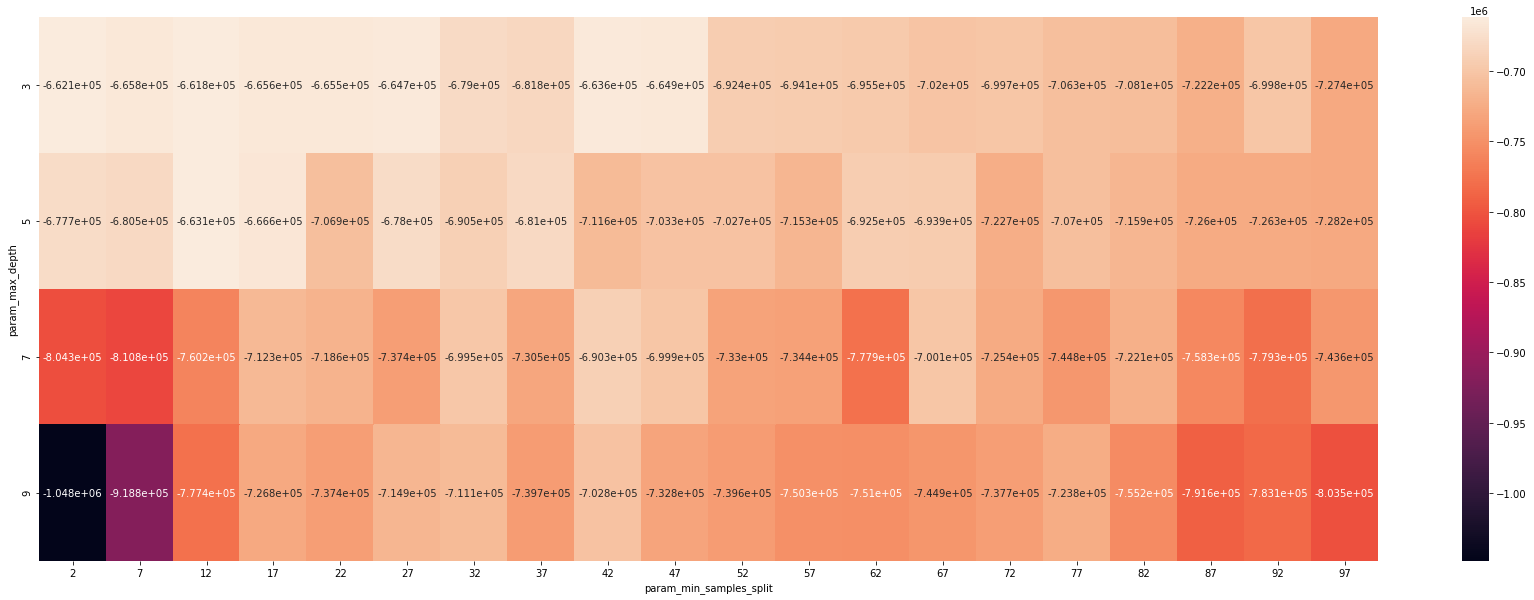
\includegraphics[width=12cm]{images/hyper_parameter_tunning}
    \caption{Tepelná mapa skóre natrénovaného modelu (regresia) podľa zvolených parametrov. Na osi $x$ je parameter \textit{min samples split} na osi $y$ je parameter \textit{max depth}. Farba vyjadruje skóre modelu (neg. RMSE). Čím je farba bledšia, tým je chyba modelu nižšia.}
    \label{fig:hyper_parameter_tunning}
\end{figure}
 
Pri optimalizácii hyper-parametrov sme použili krížovú validáciu s $k=5$ (tj. dátová sada bola rozdelená na 5 častí).

Takto sa nám pre obe úlohy podarilo zlepšiť natrénované modely, avšak niektoré len minimálne (Tab. \ref{tab:hyper_parameter_tunning}).

\begin{center}
    \begin{table}[]
        \begin{tabular}{|l|l|l|l|r|r|}
        \hline
        \multicolumn{1}{|c|}{Úloha} & \multicolumn{1}{c|}{Predikovaný atribút} & \multicolumn{1}{c|}{Model} & \multicolumn{1}{c|}{Metrika} & \multicolumn{1}{c|}{Pred} & \multicolumn{1}{c|}{Po} \\ \hline
        Klasifikácia                & Position (4)                             & GBT                        & F1 micro/macro               & 0.893/0.904                   & 0.896/0.906                                  \\ \hline
        Klasifikácia                & Position (13)                            & GBT                        & F1 micro/macro               & 0.698/0.526                   & 0.696/0.535                                  \\ \hline
        Regresia                    & Value                                    & GBT                        & RMSE                         & 0.529 M                       & 0.506 M                                      \\ \hline
        \end{tabular}
        \\
        \caption{\label{tab:hyper_parameter_tunning} Porovnanie úspešnosti modelov pred a po optimalizácii hyper-parametrov s použitím \textbf{všetkých} atribútov.}
    \end{table}
\end{center}

\subsection{Ďaľšie experimenty}

S vybranými najoptimálnejšími parametrami sme následne experimentovali s oversamplingom, ktorý model vždy zhoršil. Taktiež sme sa pokúsili natrénovať čo najjednoduchší model - tj. použiť čo najmenej atribútov, taký model je potom ľahšie interpretovateľný.
V prípade klasifikácie do `Position 4` sa použítím iba 13 atribútov (z 52) skóre zhoršilo iba minimálne z \textit{0.896/0.906} (f1 micro/macro) na \textit{0.873/0.887}. V prípade klasifikácie do `Position 13` bol tento trend podobný. Matice zmätenia najlepšieho modelu je podobná matici zmätenia logistickej regresie z Obr. \ref{fig:confusion_matrix_position_4} preto ju nebudeme vizualizovať.

V prípade regresie sa nám dokonca podarilo natrénovať lepší model s \\\textit{RMSE=0,474} (Obr. \ref{fig:gbt_regression}) (predtým \textit{RMSE=0.506}) s použítím 33 namiesto všetkých (71 - atribútov pre regresiu je viac pretože obsahujú aj herné pozície hráča) atribútov. S použitím iba dvoch atribútov - veku hráča (stĺpec `Age`) a jeho celkového hodnotenia (stĺpec `Overall`) sme dosiahli \textit{RMSE=1}, teda iba z týchto dvoch atribútov sme vedeli predpovedať trhovú hodnotu hráča s chybou 1 milión.

\begin{figure}[htp]
    \centering
    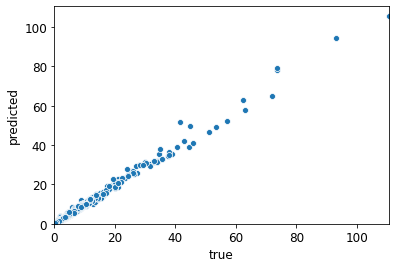
\includegraphics[height=5cm]{images/gbt_regression}
    \caption{Predikované hodnoty hráčov a reálne hodnoty hráčov (v miliónoch) našim najlepším modelom. (\textit{RMSE = 0,474}).}
    \label{fig:gbt_regression}
\end{figure}


\section{Zhodnotenie}

Oproti našim prvotným baseline modelom v sekciách \ref{classification}  a \ref{regression} sa nám podarilo zlepšiť v oboch úlohách. V klasifikácií do trinástich pozícií sa nám nepodarilo dosiahnuť tak dobré výsledky ako pri klasifikácii do štyroch. Celkovo sa nám podarilo:
\begin{itemize}
    \item natrénovať model na predikciu hodnoty hráča s \textit{RMSE = 0,474} (v miliónoch)
    \item natrénovať model na predikciu hodnoty hráča iba z dvoch atribútov s \textit{RMSE = 1} (hodnota je v miliónoch)
    \item natrénovať model na klasifikáciu do 4 základných herných pozícií s úspešnosťami \textit{0.896/0.906} (f1 micro/macro)
    \item so 100\% úspešnosťou klasifikovať brankárov
    \item natrénovať všetky modely iba zo schopností hráča a jeho charakteristík
    \item natrénovať jednoduchšie modely s menej atribútami a s porovnateľnou úspešnosťou oproti použitiu všetkých atribútov
\end{itemize}

S príbuznými prácami sa \textbf{nemáme ako porovnávať}, síce sa zaoberajú pozíciou hráča, ale tak, že hľadajú ktoré atribúty sú vyznamné pre danú pozíciu hráča. Taktiež používajú inú dátovú sadu (zo staršej verzie hry). Práce, ktoré sa zaoberajú klasifikáciou pozície hráča zas používajú rozdielnu dátovú sadu s rozdielnymi atribútmi.

\section{Future Work}

Identifikovali sme nasledovné možné vylepšenia tejto práce:

\begin{itemize}
    \item hyper-parameter tunning pomocou prírodou inšpirovaných algoritmov, bayesovskej optimalizácie (angl. Bayesian optimization) alebo náhodného hľadania (angl. random search) namiesto grid search
    \item feature enginnering - napr. polynomial features
    \item interpretovanie výsledkov s cieľom zistiť kde (na akých hráčoch s akými atribútmi) sa model mýli
\end{itemize}

\newpage

\bibliographystyle{splncs04}
\bibliography{references}


\end{document}
